\chapter{System Design and Analysis}

\section{Introduction}

The Online Exam Proctoring Platform employs a three-tier architecture: React.js frontend, Flask backend, and MySQL database. This chapter presents system design diagrams (flowcharts, workflow, use case, activity, sequence, data flow, and entity-relationship) illustrating the platform's architecture and operational flow. The system integrates YOLOv8n and MediaPipe for AI proctoring, WebRTC for video streaming, Socket.IO for real-time communication, and JWT authentication for secure access control.

\section{System Architecture Overview}

The platform implements a modular three-tier architecture: \textbf{Frontend} (React.js v18+, Tailwind CSS, WebRTC, Socket.IO client), \textbf{Backend} (Flask Python 3.8+, JWT authentication, Socket.IO server, YOLOv8n/MediaPipe AI processing), and \textbf{Database} (MySQL 8.0+ with InnoDB, 21 normalized tables, AES-256 encryption). Table 3.1 summarizes technical specifications:

\begin{table}[ht]
\centering
\caption{System Architecture Technical Specifications}
\label{tab:tech_specs}
\begin{tabular}{|l|l|p{7cm}|}
\hline
\textbf{Layer} & \textbf{Component} & \textbf{Technology/Specification} \\
\hline
\multirow{5}{*}{Frontend} & Framework & React.js v18+ \\
\cline{2-3}
& Styling & Tailwind CSS \\
\cline{2-3}
& Video Streaming & WebRTC (DTLS-SRTP encryption) \\
\cline{2-3}
& Real-time Events & Socket.IO client \\
\cline{2-3}
& AI Processing & YOLOv8n (416x416, 6-7 FPS), MediaPipe (468 landmarks) \\
\hline
\multirow{4}{*}{Backend} & Framework & Flask (Python 3.8+) RESTful API \\
\cline{2-3}
& Architecture & Blueprints (modular routing) \\
\cline{2-3}
& Authentication & JWT (RFC 7519) with RBAC \\
\cline{2-3}
& Real-time Server & Socket.IO server (<150ms latency) \\
\hline
\multirow{4}{*}{Database} & DBMS & MySQL 8.0+ (InnoDB engine) \\
\cline{2-3}
& Tables & 21 normalized entities \\
\cline{2-3}
& Relationships & 40+ foreign key constraints \\
\cline{2-3}
& Encryption & AES-256 at rest, TLS in transit \\
\hline
\multirow{3}{*}{Security} & Password Hashing & bcrypt \\
\cline{2-3}
& Data Protection & GDPR, CCPA, FERPA compliant \\
\cline{2-3}
& Network Security & HTTPS/TLS, DTLS-SRTP \\
\hline
\end{tabular}
\end{table}

\section{Flowchart}

The system flowchart illustrates the complete examination lifecycle from authentication through submission. Key processes include: \textbf{Authentication} (login validation, JWT generation, role-based dashboard redirect), \textbf{Exam Initialization} (dual-camera setup via WebRTC, AI model loading), \textbf{Continuous Monitoring} (6-7 FPS frame capture, YOLOv8n object detection, MediaPipe facial analysis, violation logging with screenshot evidence, auto-ban at 5 violations), and \textbf{Submission/Grading} (automated MCQ grading, manual CQ grading, results storage). Figure 3.1 presents the complete flowchart.

\begin{figure}[ht]
    \centering
    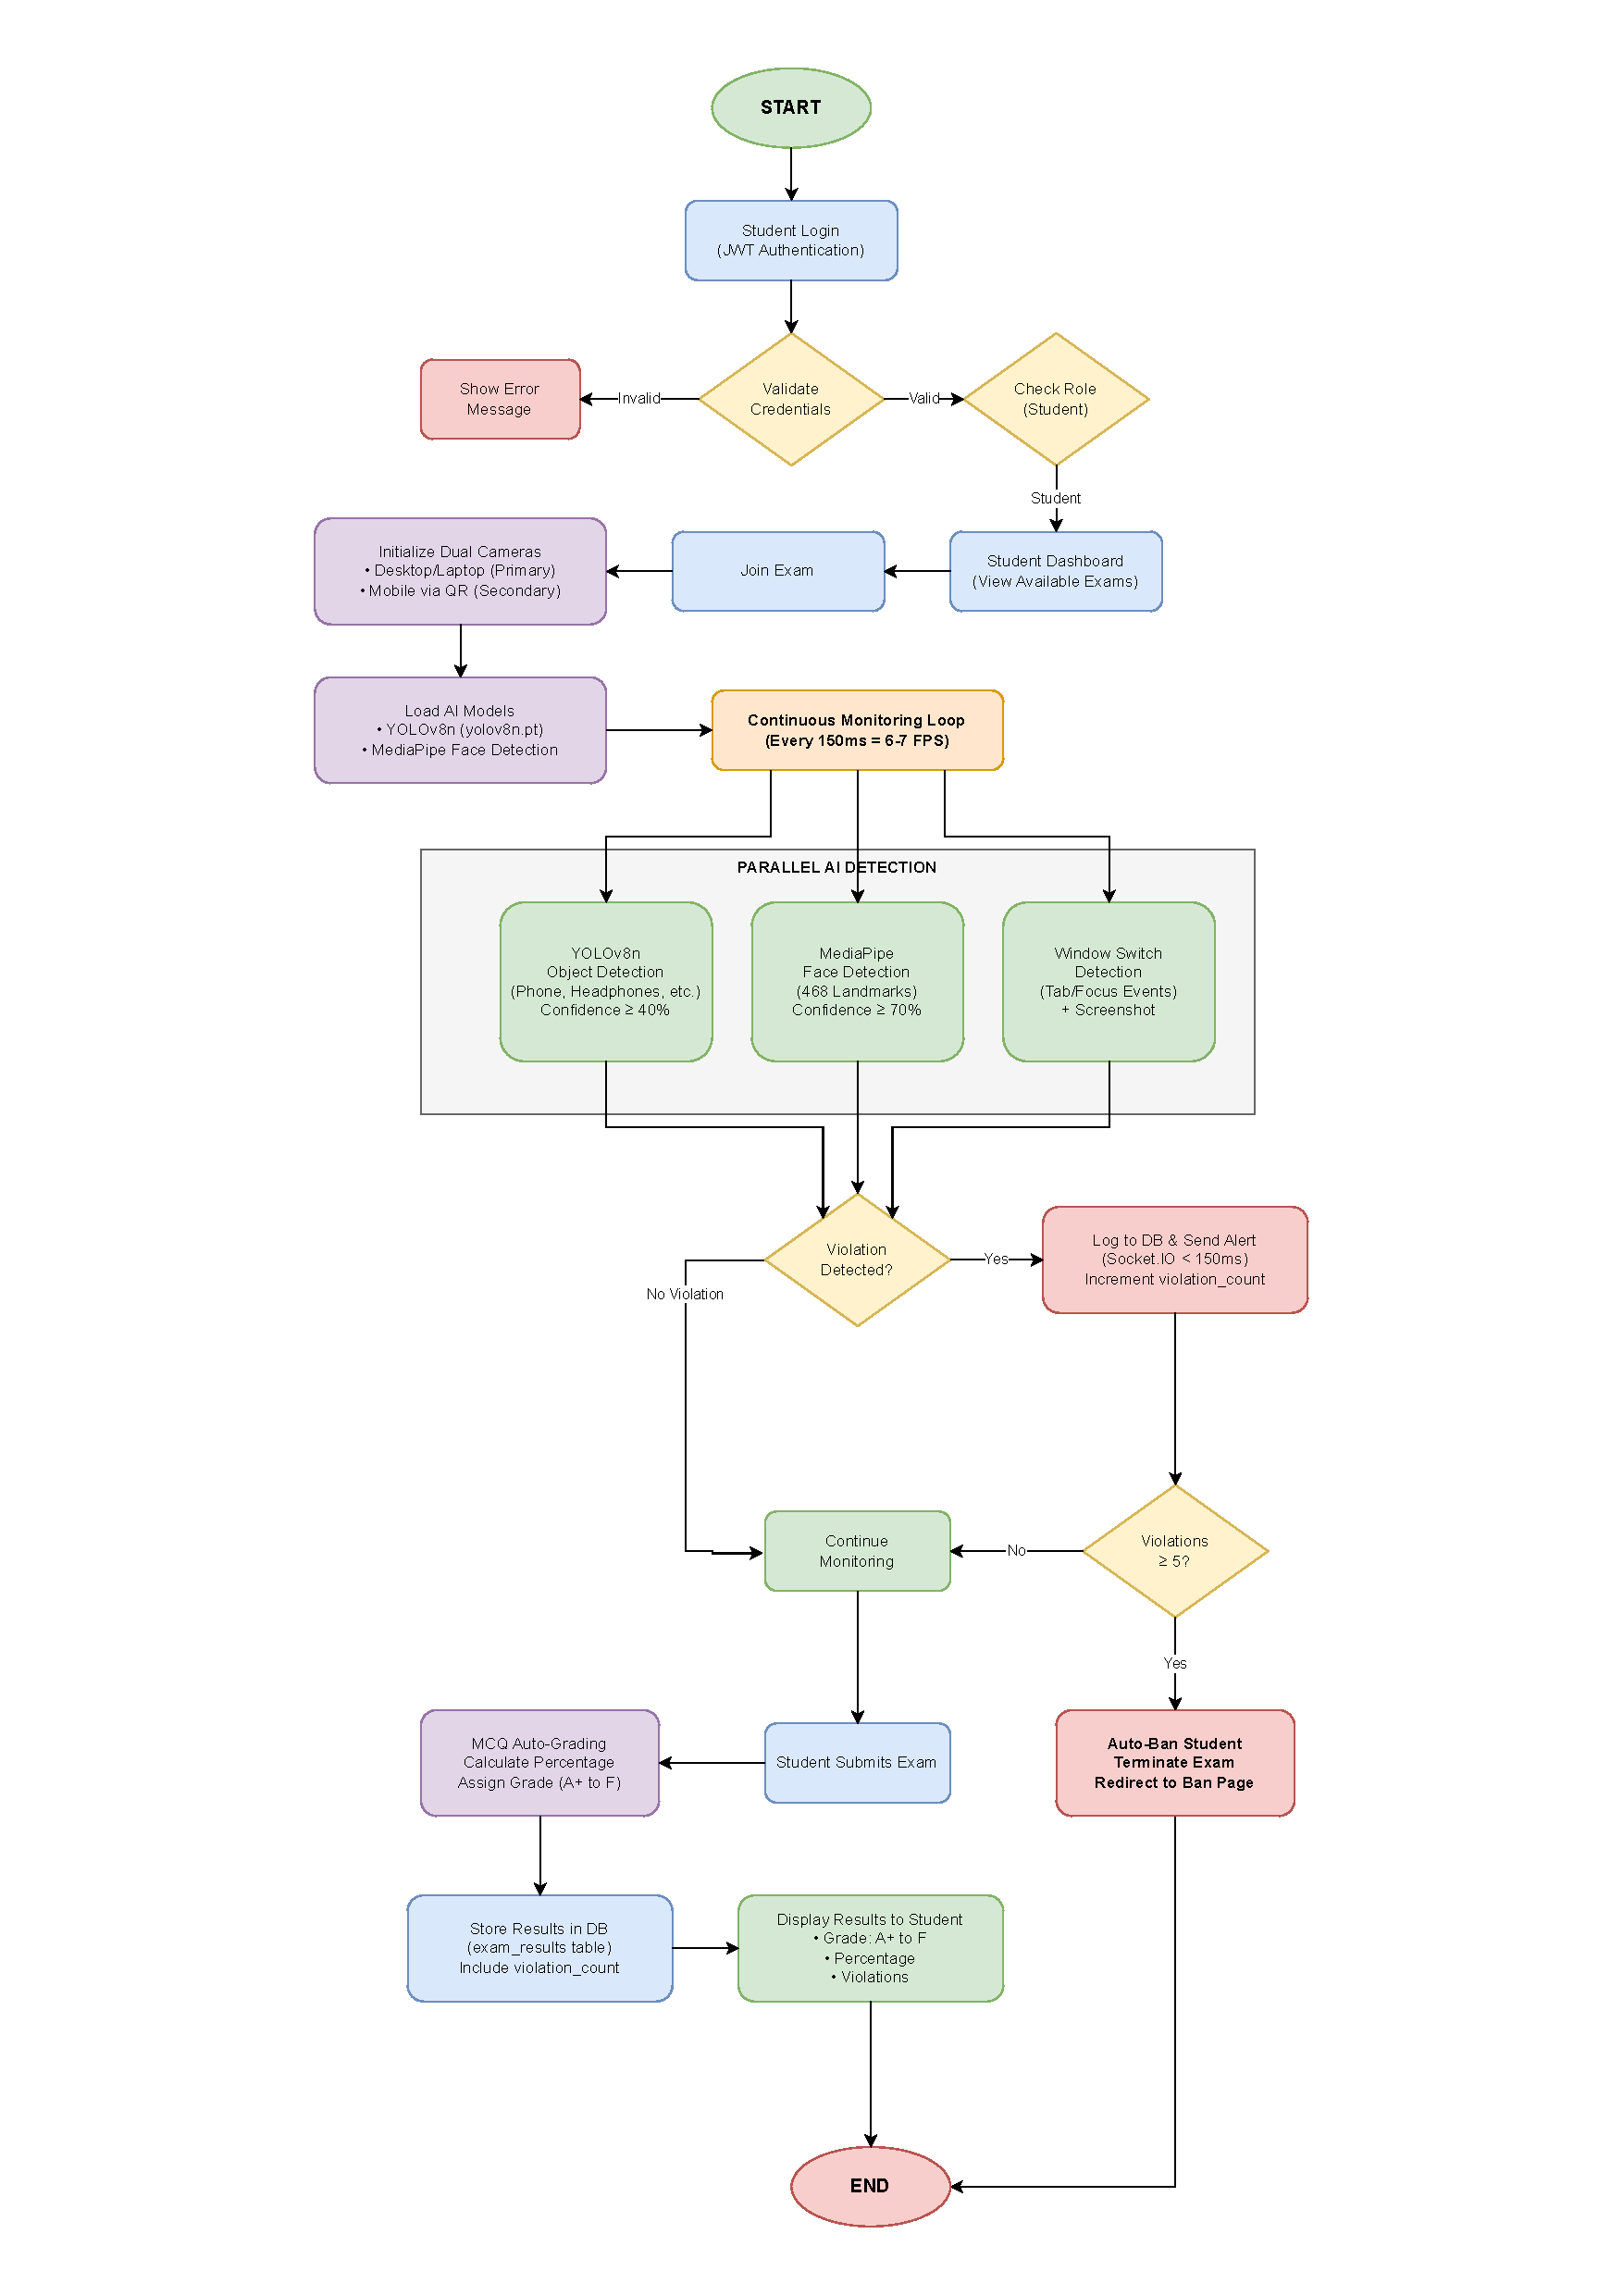
\includegraphics[width=\textwidth]{Chap3/flowchart}
    \caption{AI-Powered Online Exam Proctoring System Flowchart}
    \label{fig:flowchart}
\end{figure}

\section{Workflow Diagram}

The Five-Phase Exam Lifecycle Workflow (Figure 3.2) represents the examination process from creation to results: \textbf{Phase 1 - Exam Creation:} Teacher defines metadata, creates MCQ/CQ questions, schedules exam, automated notifications sent 10 minutes before start. \textbf{Phase 2 - Pre-Exam:} System sends Socket.IO notifications, students verify camera permissions, teachers open proctoring dashboard. \textbf{Phase 3 - Exam Taking:} Parallel streams include student activity (QR code pairing, answering questions), AI monitoring (YOLOv8n/MediaPipe analysis, violation detection), and teacher monitoring (real-time alerts $<$150ms). \textbf{Phase 4 - Grading:} MCQ auto-graded with percentage-based grades (A+ to F), CQ manually graded by teachers. \textbf{Phase 5 - Results:} Students view marks/grades/violations, teachers access analytics and reports. Figure 3.2 illustrates the complete workflow.

\begin{figure}[ht]
    \centering
    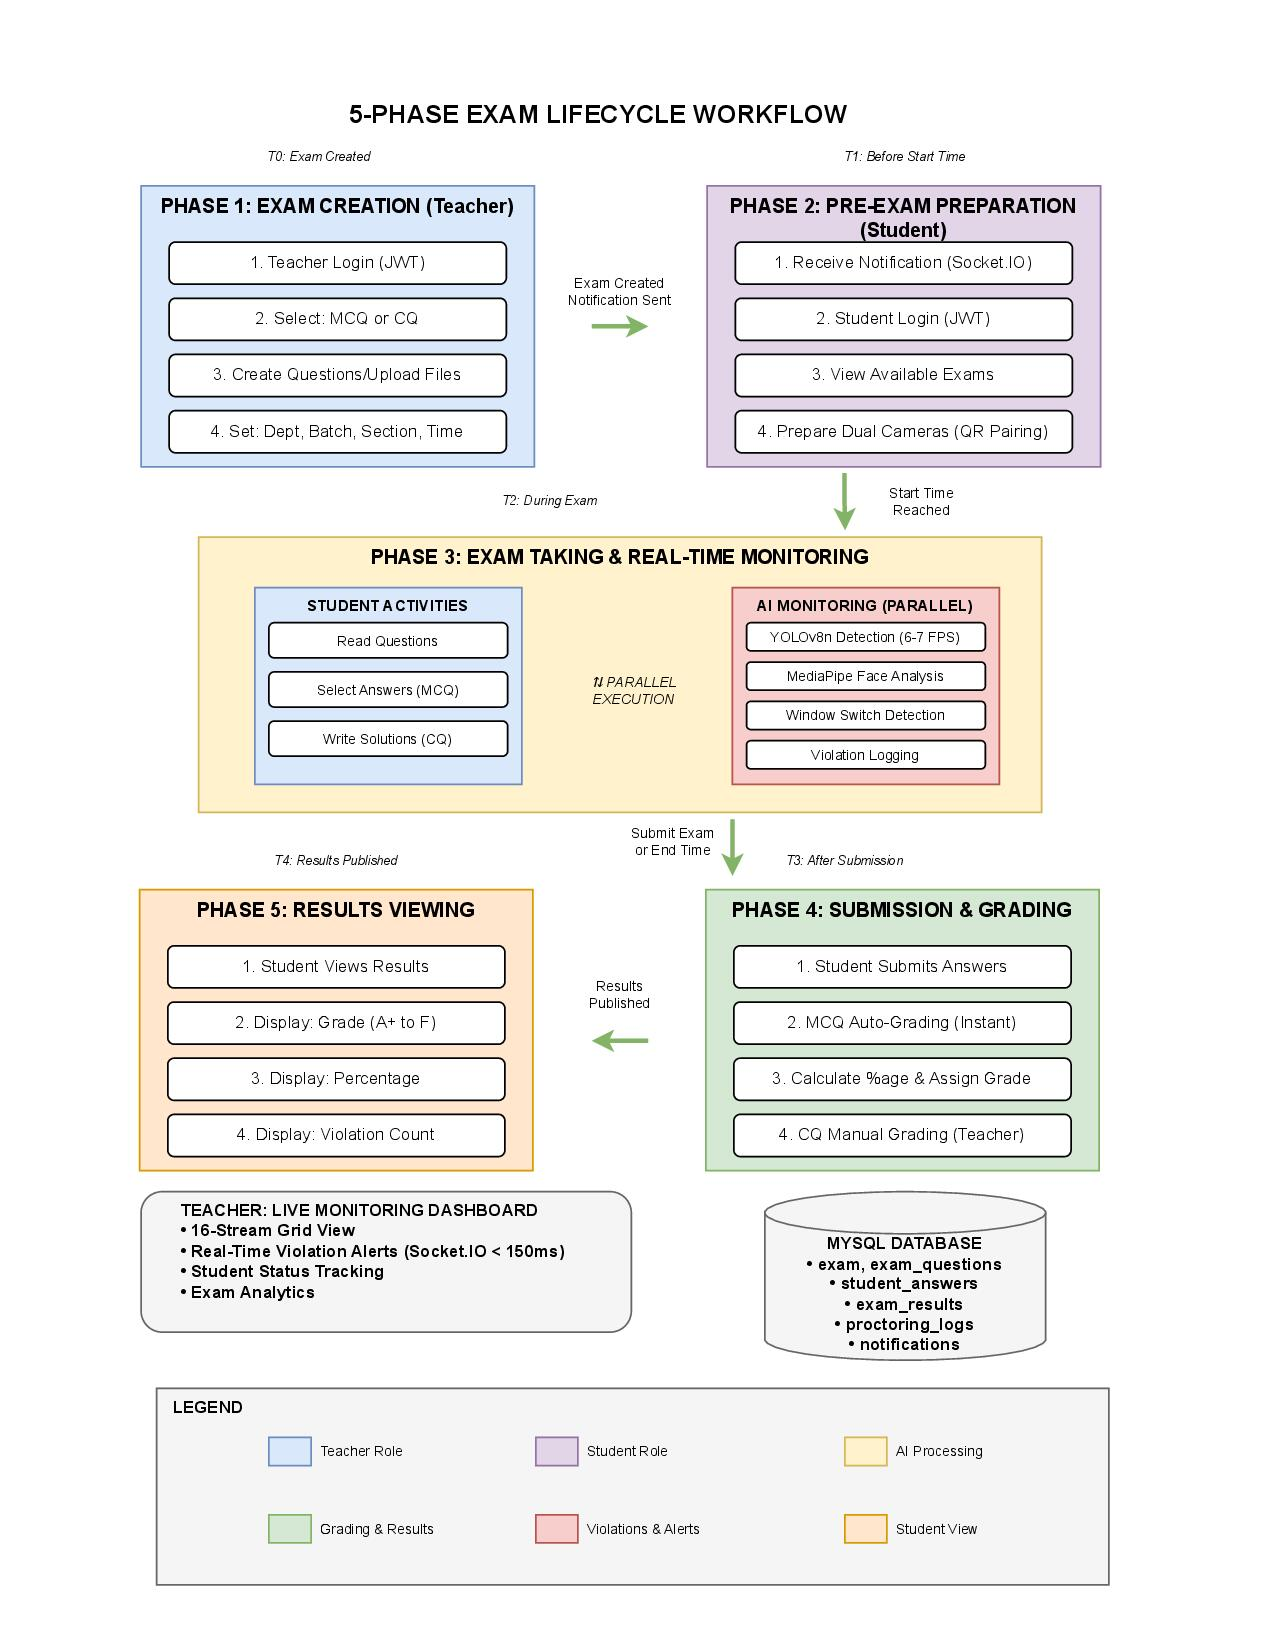
\includegraphics[width=\textwidth]{Chap3/workflow}
    \caption{Five-Phase Exam Lifecycle Workflow Diagram}
    \label{fig:workflow}
\end{figure}

\section{Use Case Diagram}

The Use Case Diagram (Figure 3.3) identifies four actors and their system interactions. \textbf{Student:} Login, join exam, initialize cameras, answer MCQ/CQ, submit exam, view results/violations, submit unban requests. \textbf{Teacher:} Create/edit/delete exams, add questions, view live proctoring dashboard, monitor violations, grade CQ answers, generate reports, manage students, approve unban requests. \textbf{Administrator:} Manage users (CRUD), configure system, manage departments/batches/sections/semesters/courses, view analytics, backup database. \textbf{AI System:} Detect objects (YOLOv8n), detect faces/multiple persons (MediaPipe), analyze gaze/head pose, classify violations, capture screenshots, send real-time alerts, log violations, auto-ban at 5 violations. Relationships include \textless\textless include\textgreater\textgreater~(mandatory sub-functionality) and \textless\textless extend\textgreater\textgreater~(optional functionality). Figure 3.3 presents the complete diagram.

\begin{figure}[ht]
    \centering
    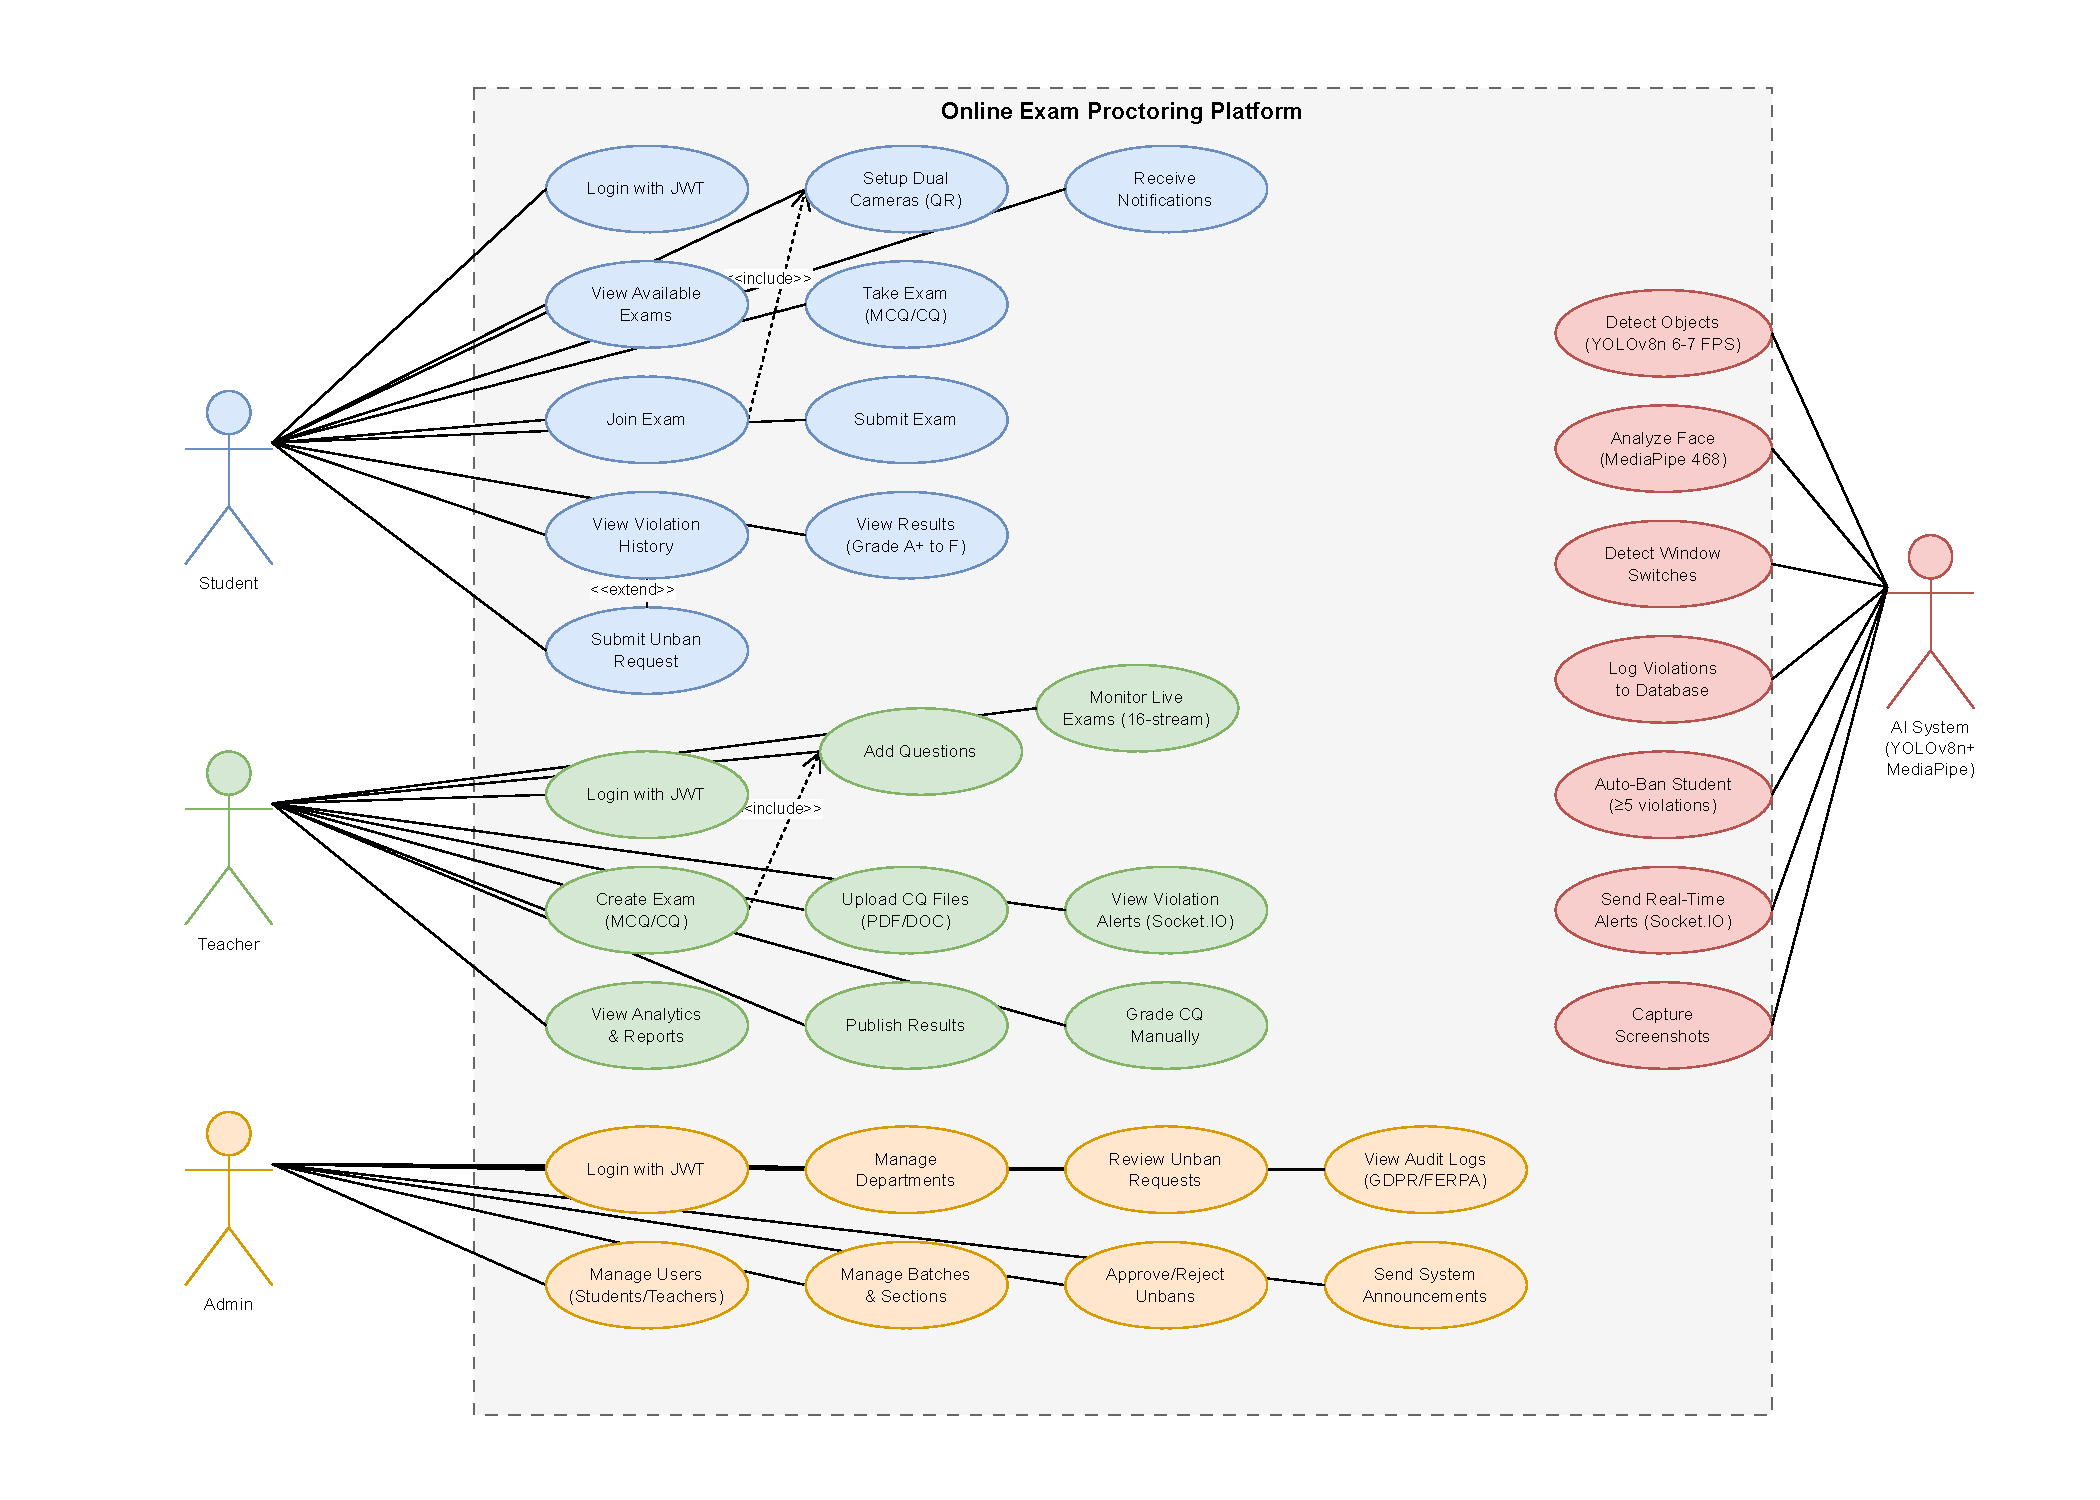
\includegraphics[width=\textwidth]{Chap3/usecase}
    \caption{Use Case Diagram - System Actors and Interactions}
    \label{fig:usecase}
\end{figure}

\section{Activity Diagram}

The Parallel Monitoring Activity Diagram (Figure 3.4) models concurrent execution during exams. \textbf{Student Swimlane:} Login $\rightarrow$ Select Exam $\rightarrow$ Initialize Cameras $\rightarrow$ Fork (begin parallel execution) $\rightarrow$ Read/Answer Questions (loop) $\rightarrow$ Submit $\rightarrow$ Join (synchronization) $\rightarrow$ View Results. \textbf{AI Monitoring Swimlane:} Fork $\rightarrow$ Capture Frame (6-7 FPS) $\rightarrow$ Run YOLOv8n/MediaPipe $\rightarrow$ Analyze Violations $\rightarrow$ Decision (violation detected?) $\rightarrow$ Screenshot/Alert/Log/Counter Increment $\rightarrow$ Decision (violations $\geq$ 5?) $\rightarrow$ Auto-ban or Continue $\rightarrow$ Loop until submission $\rightarrow$ Terminate $\rightarrow$ Join. Fork/join nodes show parallelism, diamond shapes represent decisions, cyclic paths show loops. Figure 3.4 demonstrates the parallel processing architecture.

\begin{figure}[ht]
    \centering
    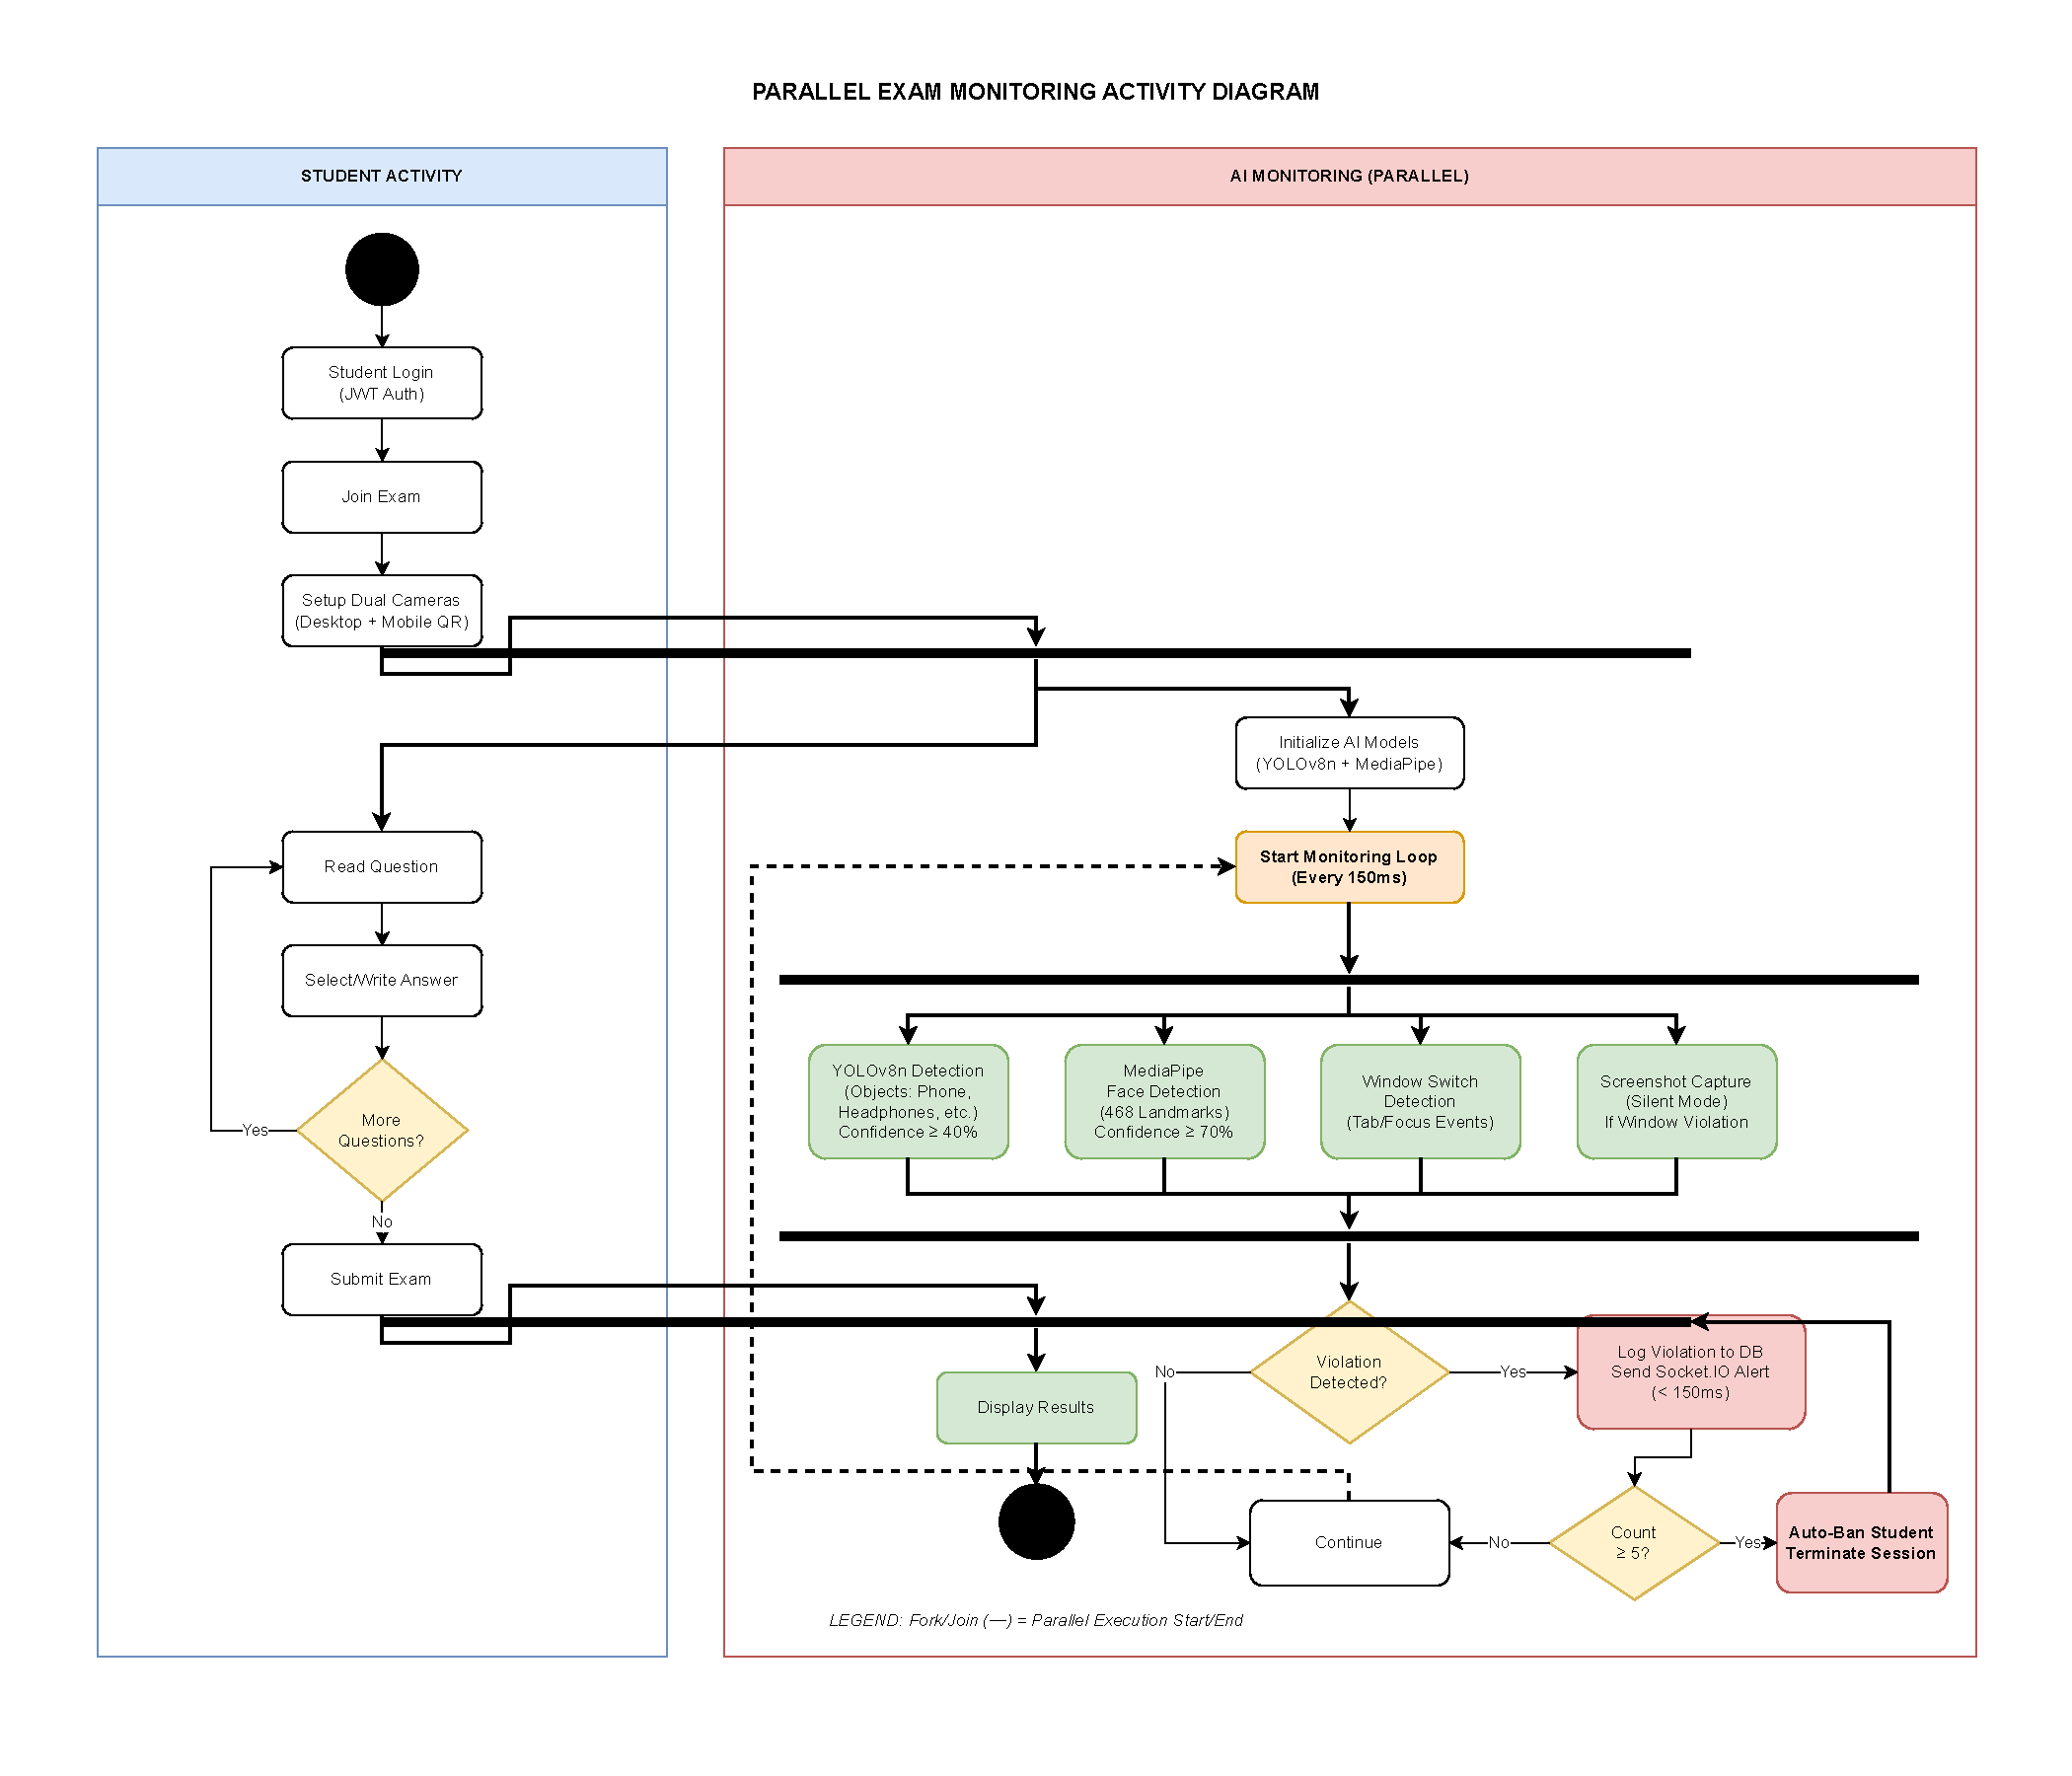
\includegraphics[width=0.95\textwidth]{Chap3/activity}
    \caption{Parallel Monitoring Activity Diagram with Swimlanes}
    \label{fig:activity}
\end{figure}

\section{Sequence Diagram}

The WebRTC and Socket.IO Sequence Diagram (Figure 3.5) captures message flow during examination sessions. Participating objects: Student, Frontend (React.js), Backend (Flask), AI Models (YOLOv8n/MediaPipe), Database (MySQL), Socket.IO, Teacher. \textbf{Authentication:} Student credentials $\rightarrow$ POST /api/auth/login $\rightarrow$ Database query $\rightarrow$ bcrypt verification $\rightarrow$ JWT token generation $\rightarrow$ Dashboard redirect. \textbf{Initialization:} GET /api/exam/\{id\} $\rightarrow$ Database retrieval $\rightarrow$ Display exam $\rightarrow$ WebRTC initialization $\rightarrow$ AI model loading. \textbf{Proctoring Loop:} Capture frame $\rightarrow$ AI processing $\rightarrow$ [ALT: Violation] POST /api/violations/log $\rightarrow$ INSERT proctoring\_logs $\rightarrow$ Socket.IO emit $\rightarrow$ Teacher alert ($<$150ms) $\rightarrow$ [LOOP: Every 150ms]. \textbf{Submission:} POST /api/exam/submit $\rightarrow$ INSERT student\_answers $\rightarrow$ Grade MCQ $\rightarrow$ Calculate marks/grade $\rightarrow$ INSERT exam\_results $\rightarrow$ Display results. Features include synchronous/asynchronous messages, lifelines, activation boxes, LOOP/ALT frames. Figure 3.5 presents complete message flow.

\begin{figure}[ht]
    \centering
    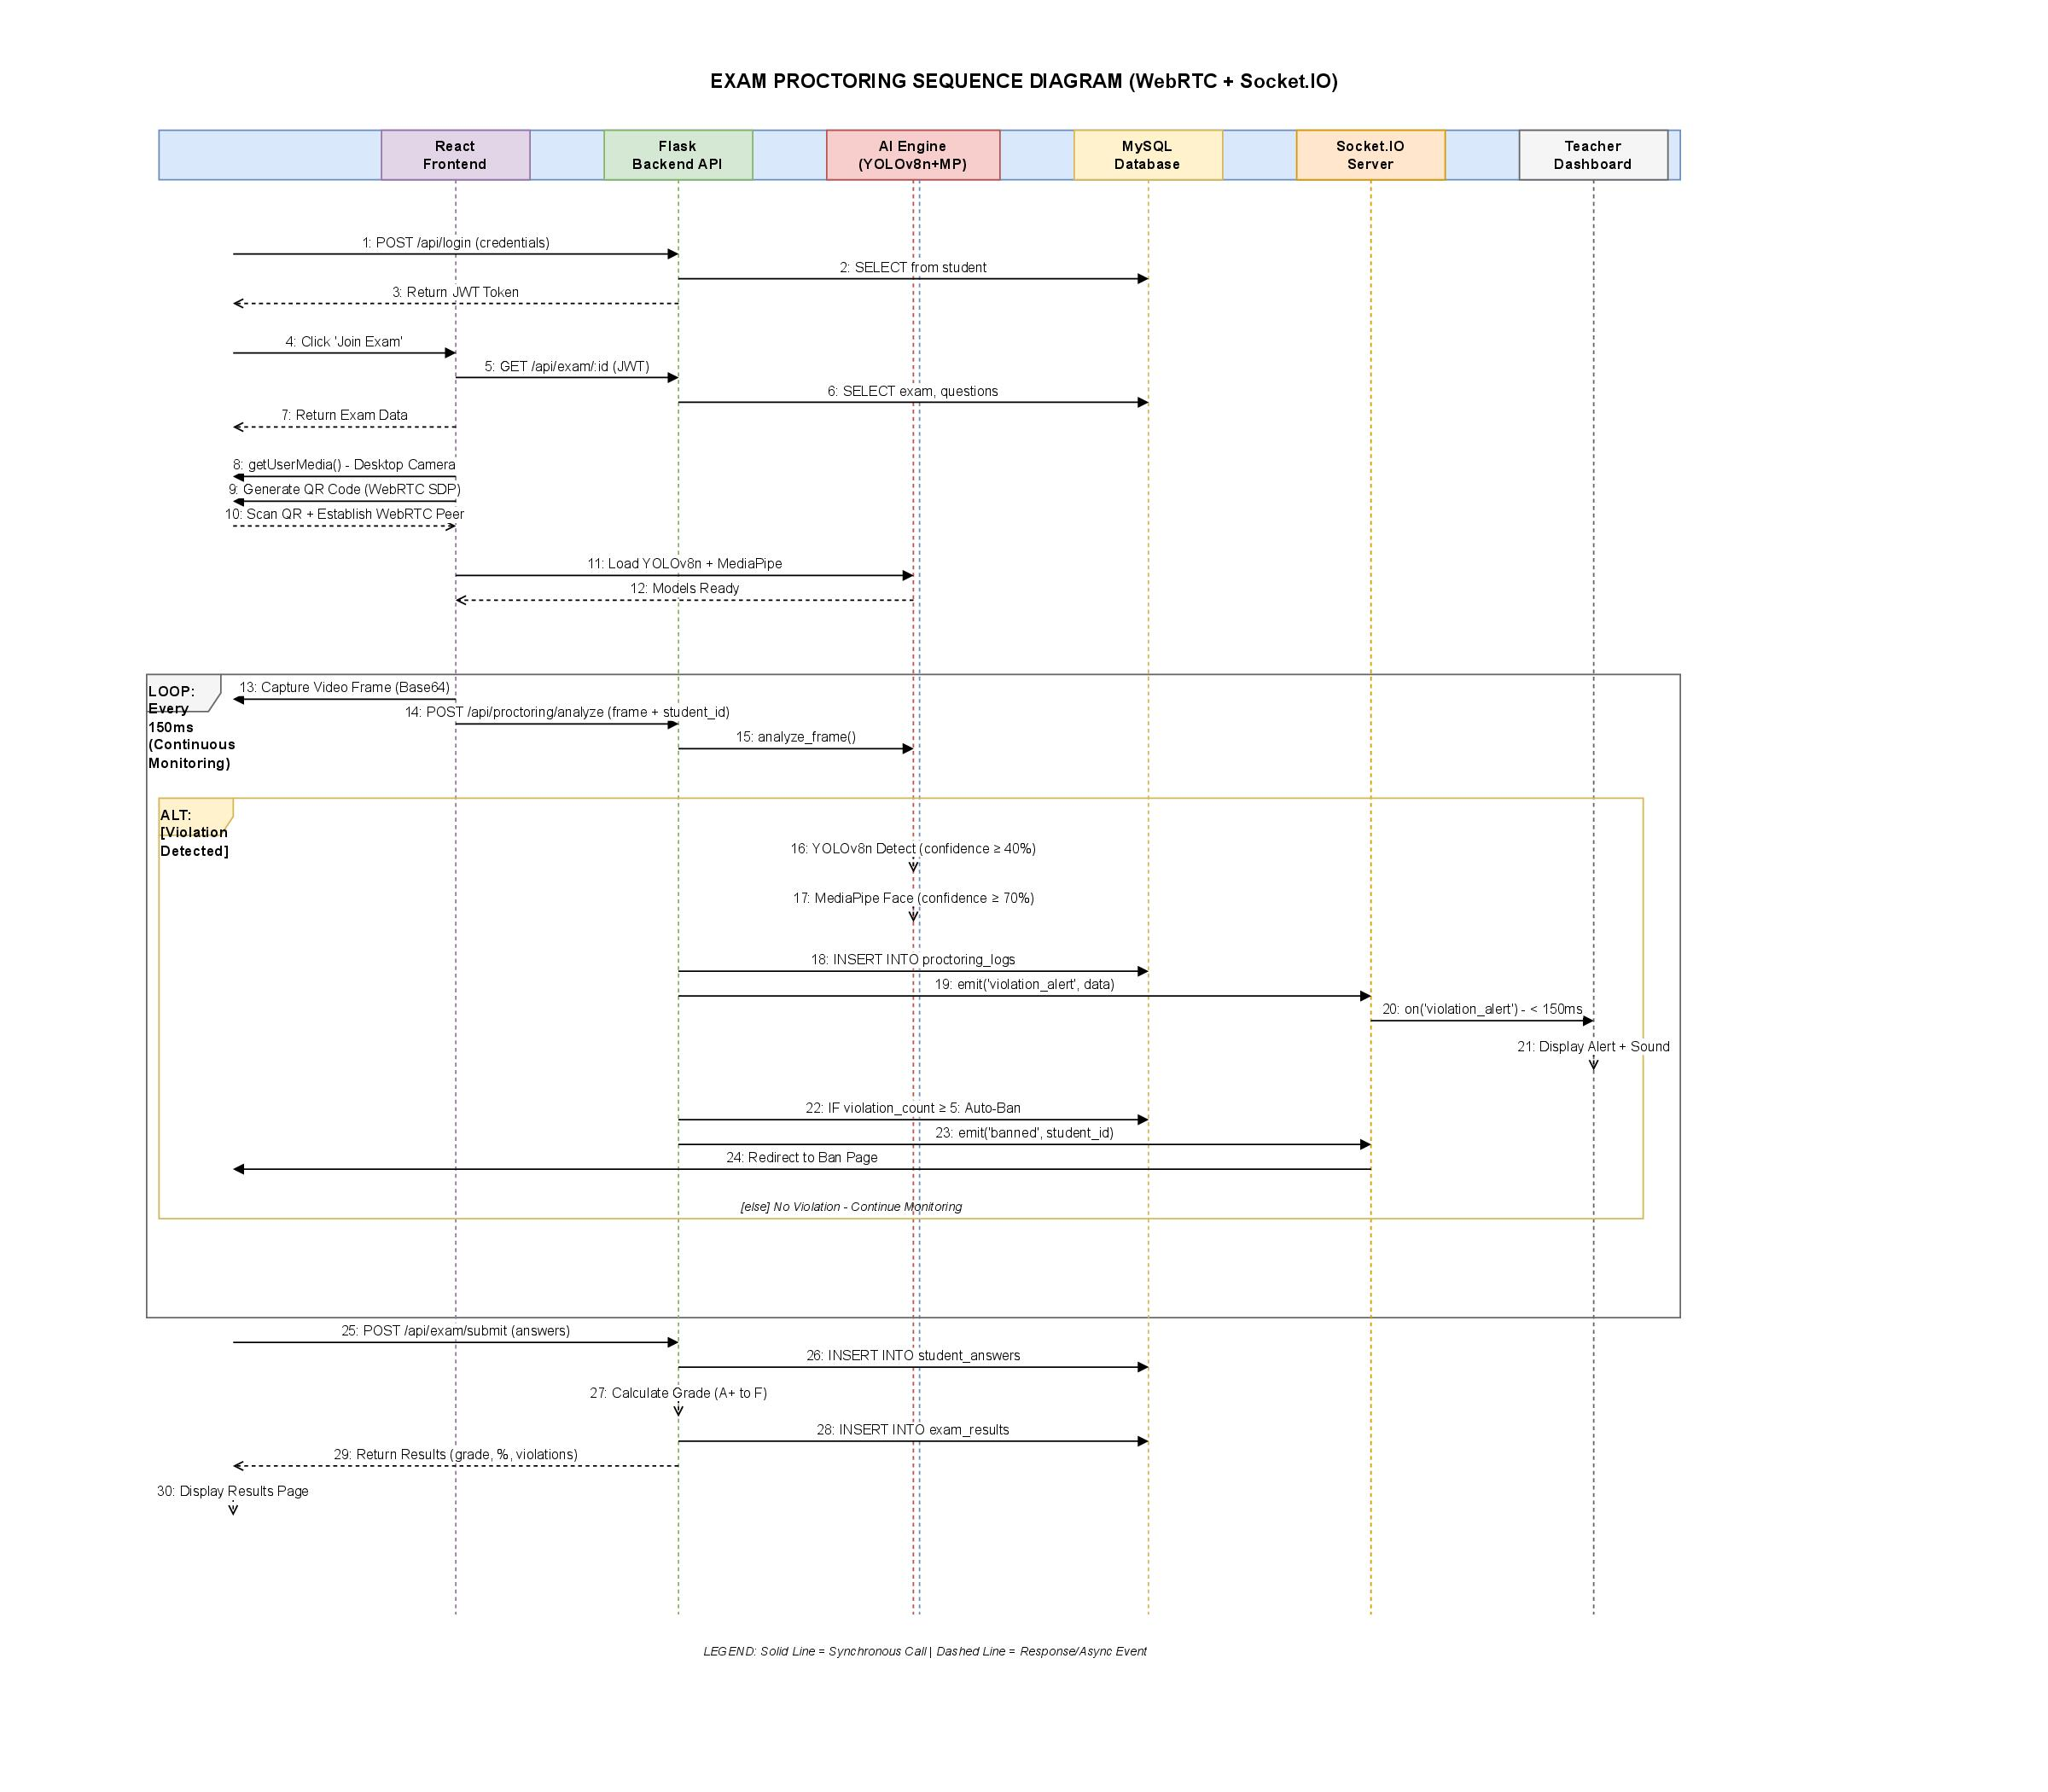
\includegraphics[width=\textwidth]{Chap3/sequence}
    \caption{WebRTC and Socket.IO Sequence Diagram - Message Flow}
    \label{fig:sequence}
\end{figure}

\section{Data Flow Diagram}

DFDs represent data movement through processes, data stores, and external entities across hierarchical levels.

\subsection{DFD Level 0 (Context Diagram)}

The Context Diagram (Figure 3.6) shows the system as a single process with four external entities: \textbf{Student} (provides credentials/answers, receives results/notifications), \textbf{Teacher} (creates exams/grades, receives violation alerts), \textbf{Administrator} (manages configuration/users, receives logs/analytics), \textbf{AI System} (exchanges video frames and detection results).

\subsection{DFD Level 1 (Process Breakdown)}

The Level 1 DFD (Figure 3.7) decomposes the system into seven processes with 20 data stores: \textbf{P1 - User Authentication} (credentials $\rightarrow$ JWT token, stores: D1-users, D2-students, D3-teachers), \textbf{P2 - Exam Management} (metadata/questions $\rightarrow$ exam records, stores: D4-exam, D5-exam\_questions, D6-exam\_files, D15-course\_name), \textbf{P3 - Real-Time Proctoring} (video frames $\rightarrow$ violation alerts, stores: D7-proctoring\_logs, D8-window\_violations, D9-banned\_students), \textbf{P4 - Answer Submission} (MCQ/CQ answers $\rightarrow$ stored responses, stores: D10-student\_answers), \textbf{P5 - Automated Grading} (answers/key $\rightarrow$ marks/grade, stores: D5, D10, D11-exam\_results), \textbf{P6 - Manual Grading} (teacher evaluation $\rightarrow$ CQ marks, stores: D10, D11), \textbf{P7 - Notification Management} (schedules/events $\rightarrow$ alerts, stores: D12-notifications, D13-recipients, D14-preferences). Additional stores: D15-D19 (academic structure), D20-unban\_requests.

% Figure 3.6 and 3.7 on same page
\begin{figure}[p]
    \centering
    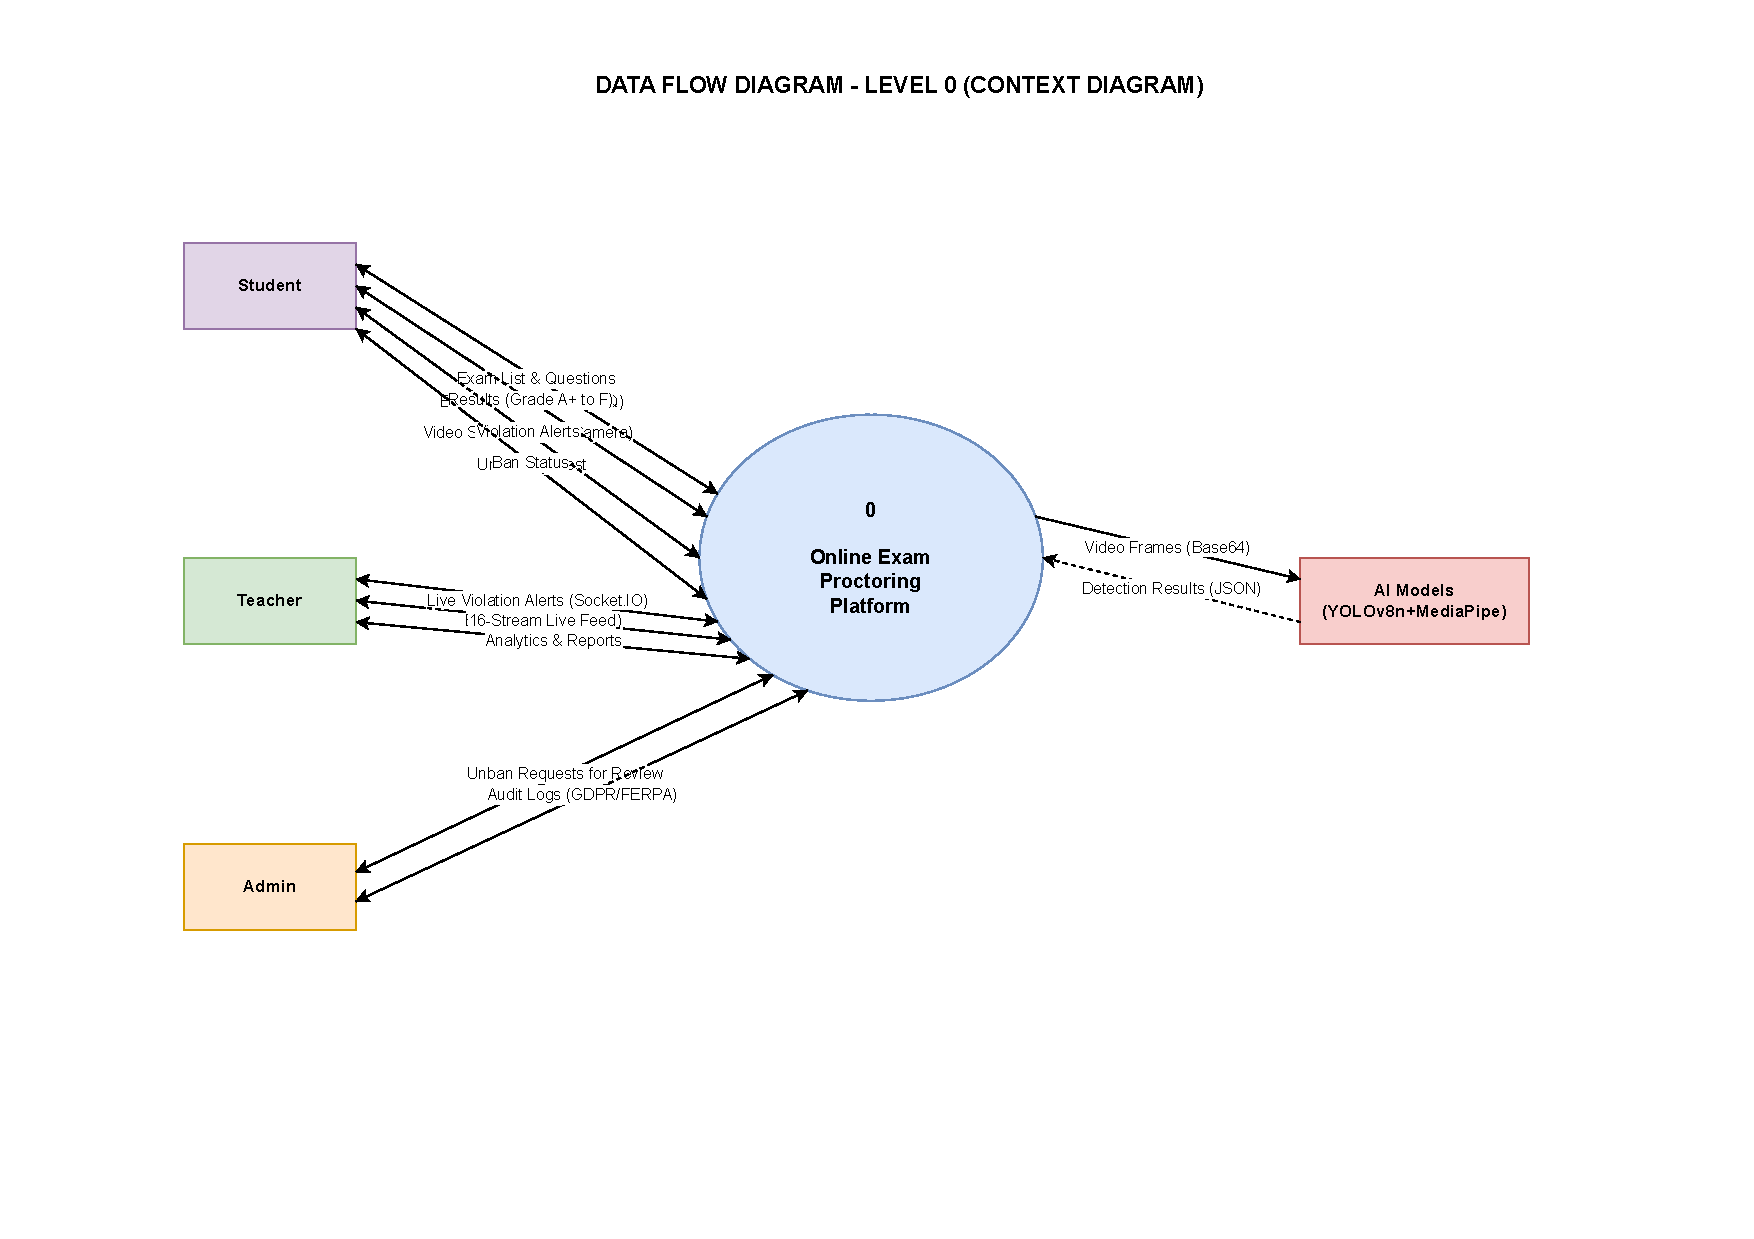
\includegraphics[width=0.85\textwidth]{Chap3/dfd_level0}
    \caption{Data Flow Diagram Level 0 - Context Diagram}
    \label{fig:dfd0}

    \vspace{1cm}

    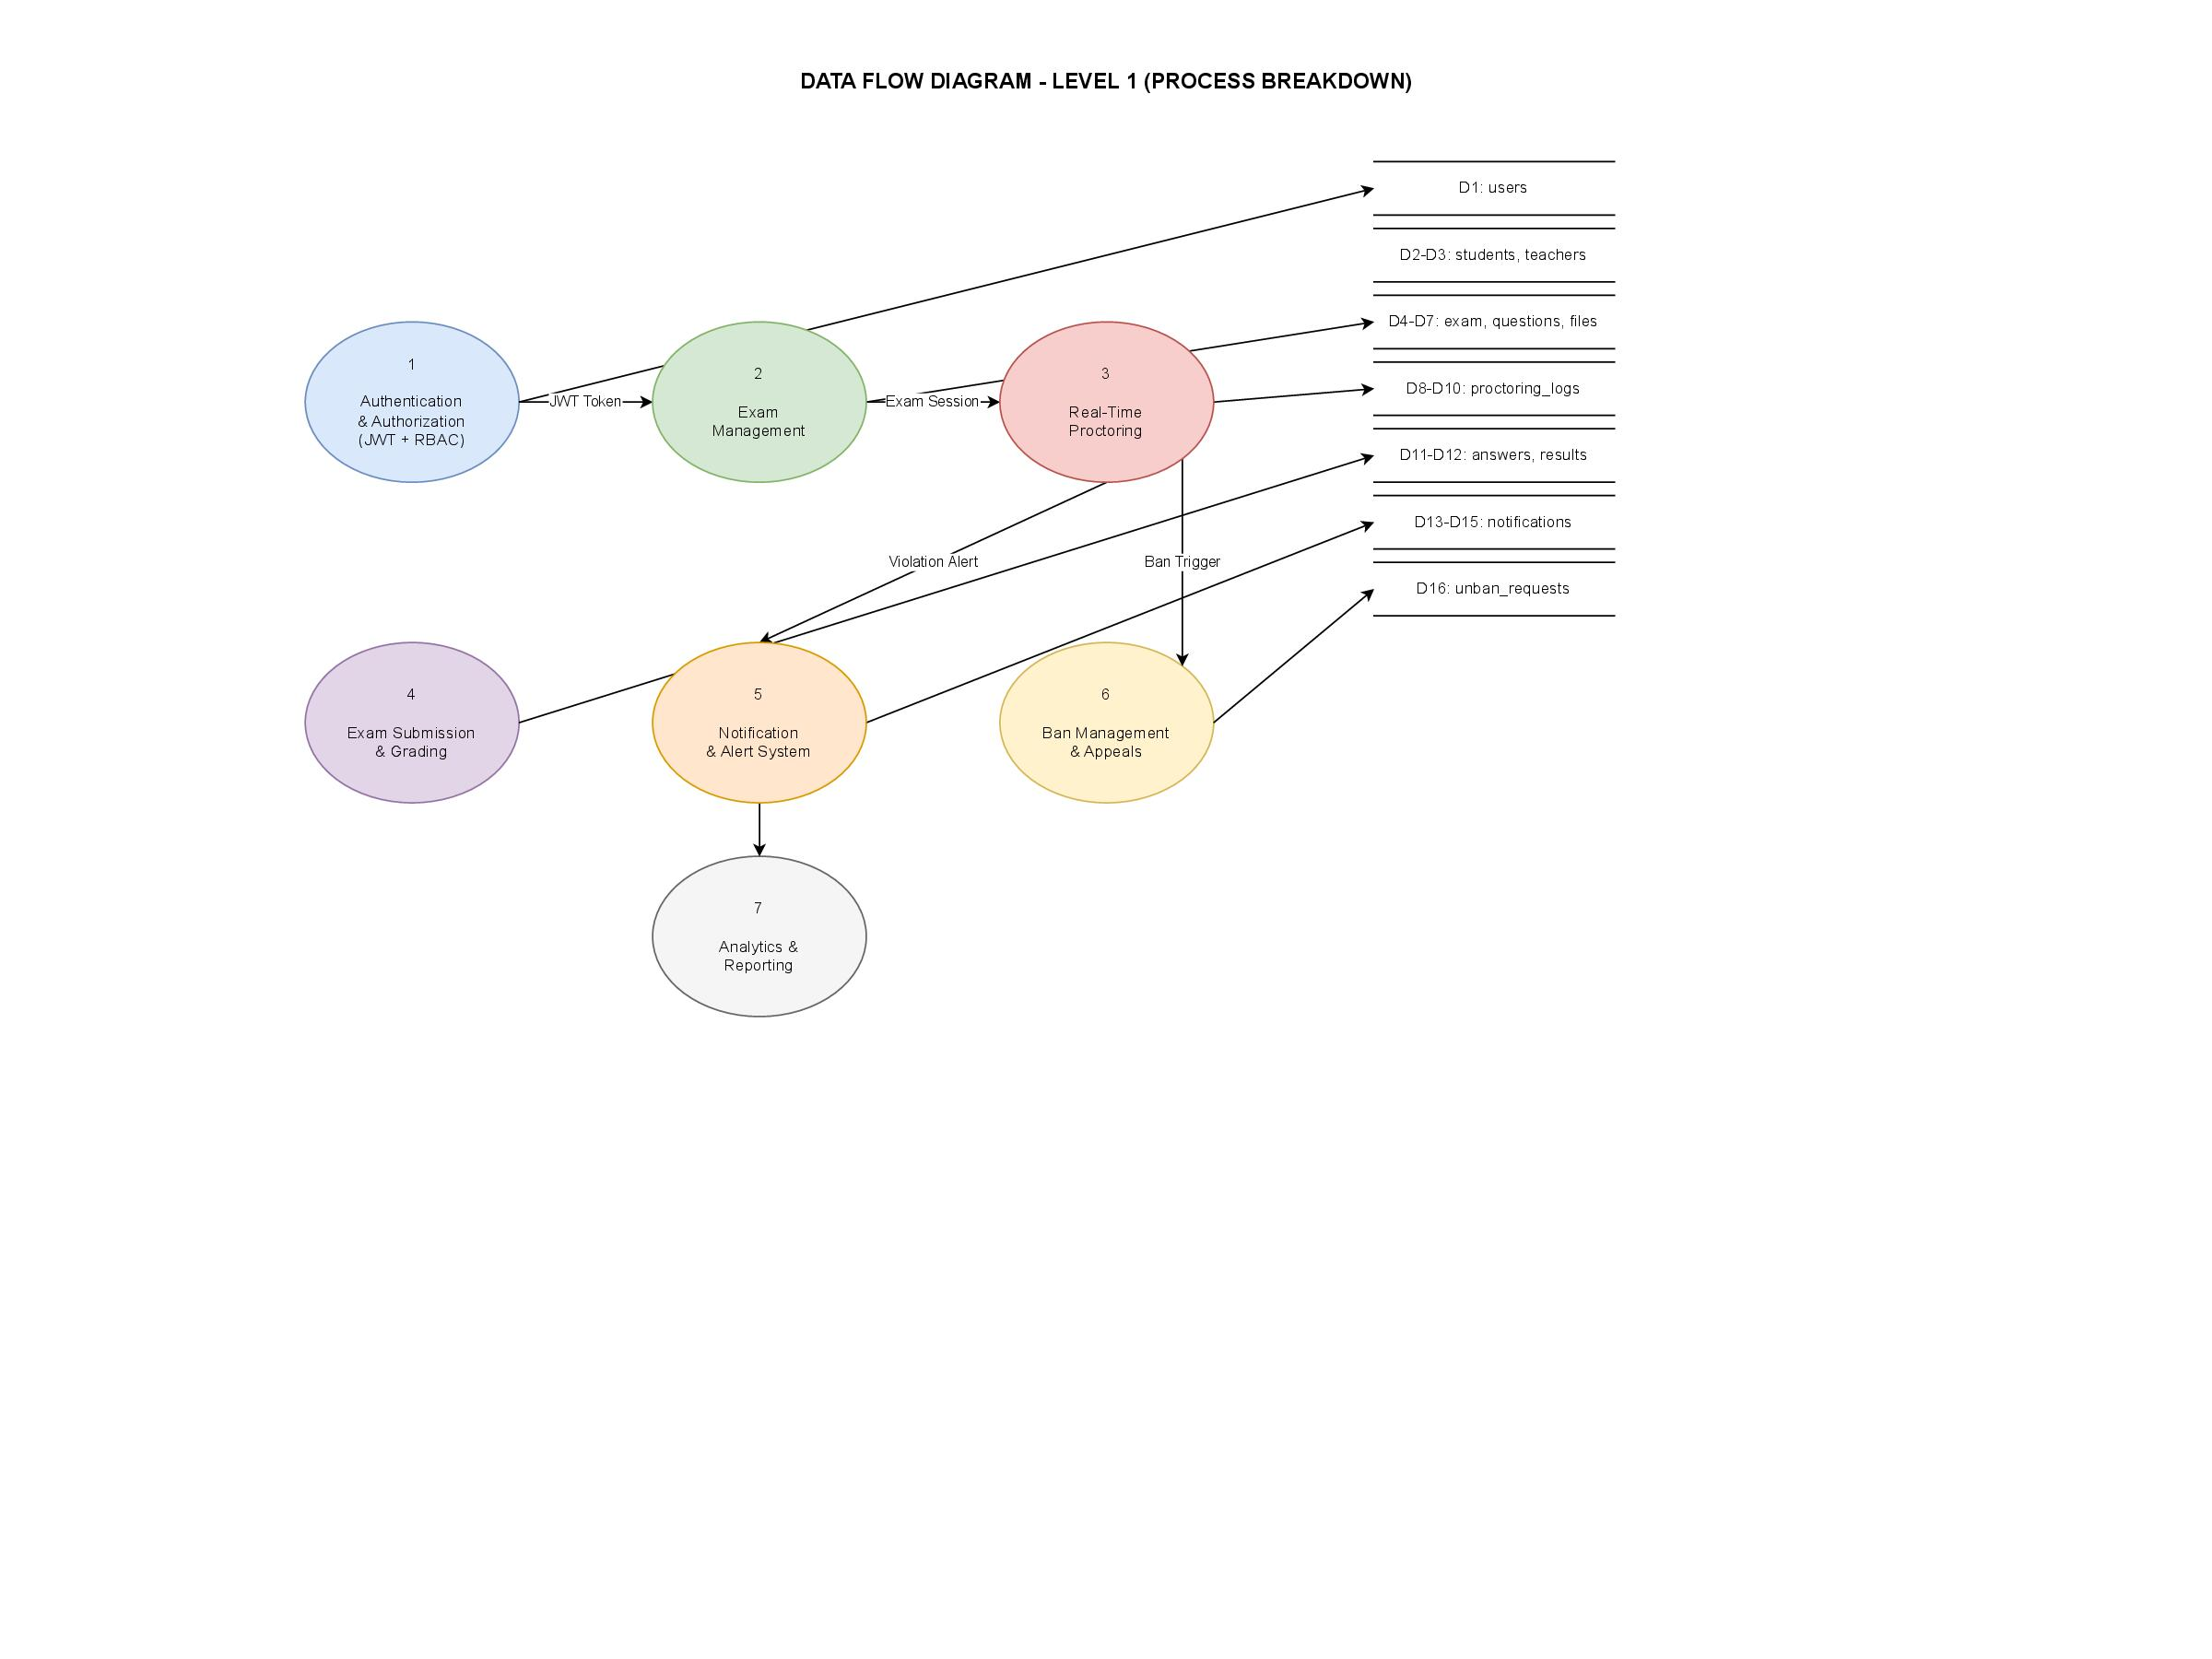
\includegraphics[width=0.85\textwidth]{Chap3/dfd_level1}
    \caption{Data Flow Diagram Level 1 - Process Breakdown}
    \label{fig:dfd1}
\end{figure}

\subsection{DFD Level 2 (Process 3 Decomposition)}

The Level 2 DFD (Figure 3.8) decomposes Process 3 (Real-Time Proctoring) into ten sub-processes: \textbf{P3.1 - Video Capture} (6-7 FPS from dual cameras), \textbf{P3.2 - Object Detection} (YOLOv8n detects prohibited items with confidence scores), \textbf{P3.3 - Face Detection} (MediaPipe analyzes facial landmarks), \textbf{P3.4 - Gaze Analysis} (estimates gaze direction/deviation), \textbf{P3.5 - Head Pose} (calculates pitch/yaw/roll angles), \textbf{P3.6 - Window Monitoring} (tracks tab/window switches), \textbf{P3.7 - Violation Classification} (determines type/priority/confidence), \textbf{P3.8 - Screenshot Capture} (Base64-encoded evidence with timestamp), \textbf{P3.9 - Real-Time Alert} (Socket.IO notification $<$150ms), \textbf{P3.10 - Violation Logging} (database storage, auto-ban at 5 violations).

\section{Entity Relationship Diagram}

The ERD (Figure 3.9) models the database structure with 21 entities across six domains: \textbf{User Management} (users, students with UNIQUE email/registration\_no, teachers), \textbf{Academic Structure} (department, batch, section, semester, course\_name), \textbf{Examination System} (exam with start/end times, exam\_questions with MCQ/CQ types, exam\_files, student\_answers, exam\_results with UNIQUE constraint on student\_id+exam\_id), \textbf{Proctoring/Security} (proctoring\_logs with Base64 screenshots, window\_violations, banned\_students, unban\_requests), \textbf{Notification System} (notifications, notification\_recipients, notification\_preferences).

\subsection{Key Relationships and Attributes}

\textbf{Relationships:} 1:N (department $\rightarrow$ students, teacher $\rightarrow$ exam, exam $\rightarrow$ exam\_questions/proctoring\_logs), M:N (students $\leftrightarrow$ exam via student\_answers, notifications $\leftrightarrow$ students via notification\_recipients), 1:1 (student $\rightarrow$ notification\_preferences, exam\_results UNIQUE on student\_id+exam\_id).

\textbf{Key Entities:} \textit{students} (PK: student\_id, bcrypt password, UNIQUE email/registration\_no, indexes on email/registration/dept-batch-section), \textit{exam} (PK: exam\_id, DATETIME start/end times, duration\_minutes, total\_marks, indexed on teacher/course/start\_time), \textit{exam\_questions} (PK: question\_id, ENUM question\_type: MCQ/CQ, option\_a-d, correct\_answer, marks), \textit{proctoring\_logs} (PK: log\_id, violation\_type, screenshot LONGTEXT Base64, DECIMAL confidence\_score, INT priority, indexed on student\_exam/type/timestamp), \textit{exam\_results} (PK: result\_id, UNIQUE student\_id+exam\_id, DECIMAL(5,2) percentage, VARCHAR(3) grade: A+ to F).

% Figure 3.8 and 3.9 on same page
\begin{figure}[p]
    \centering
    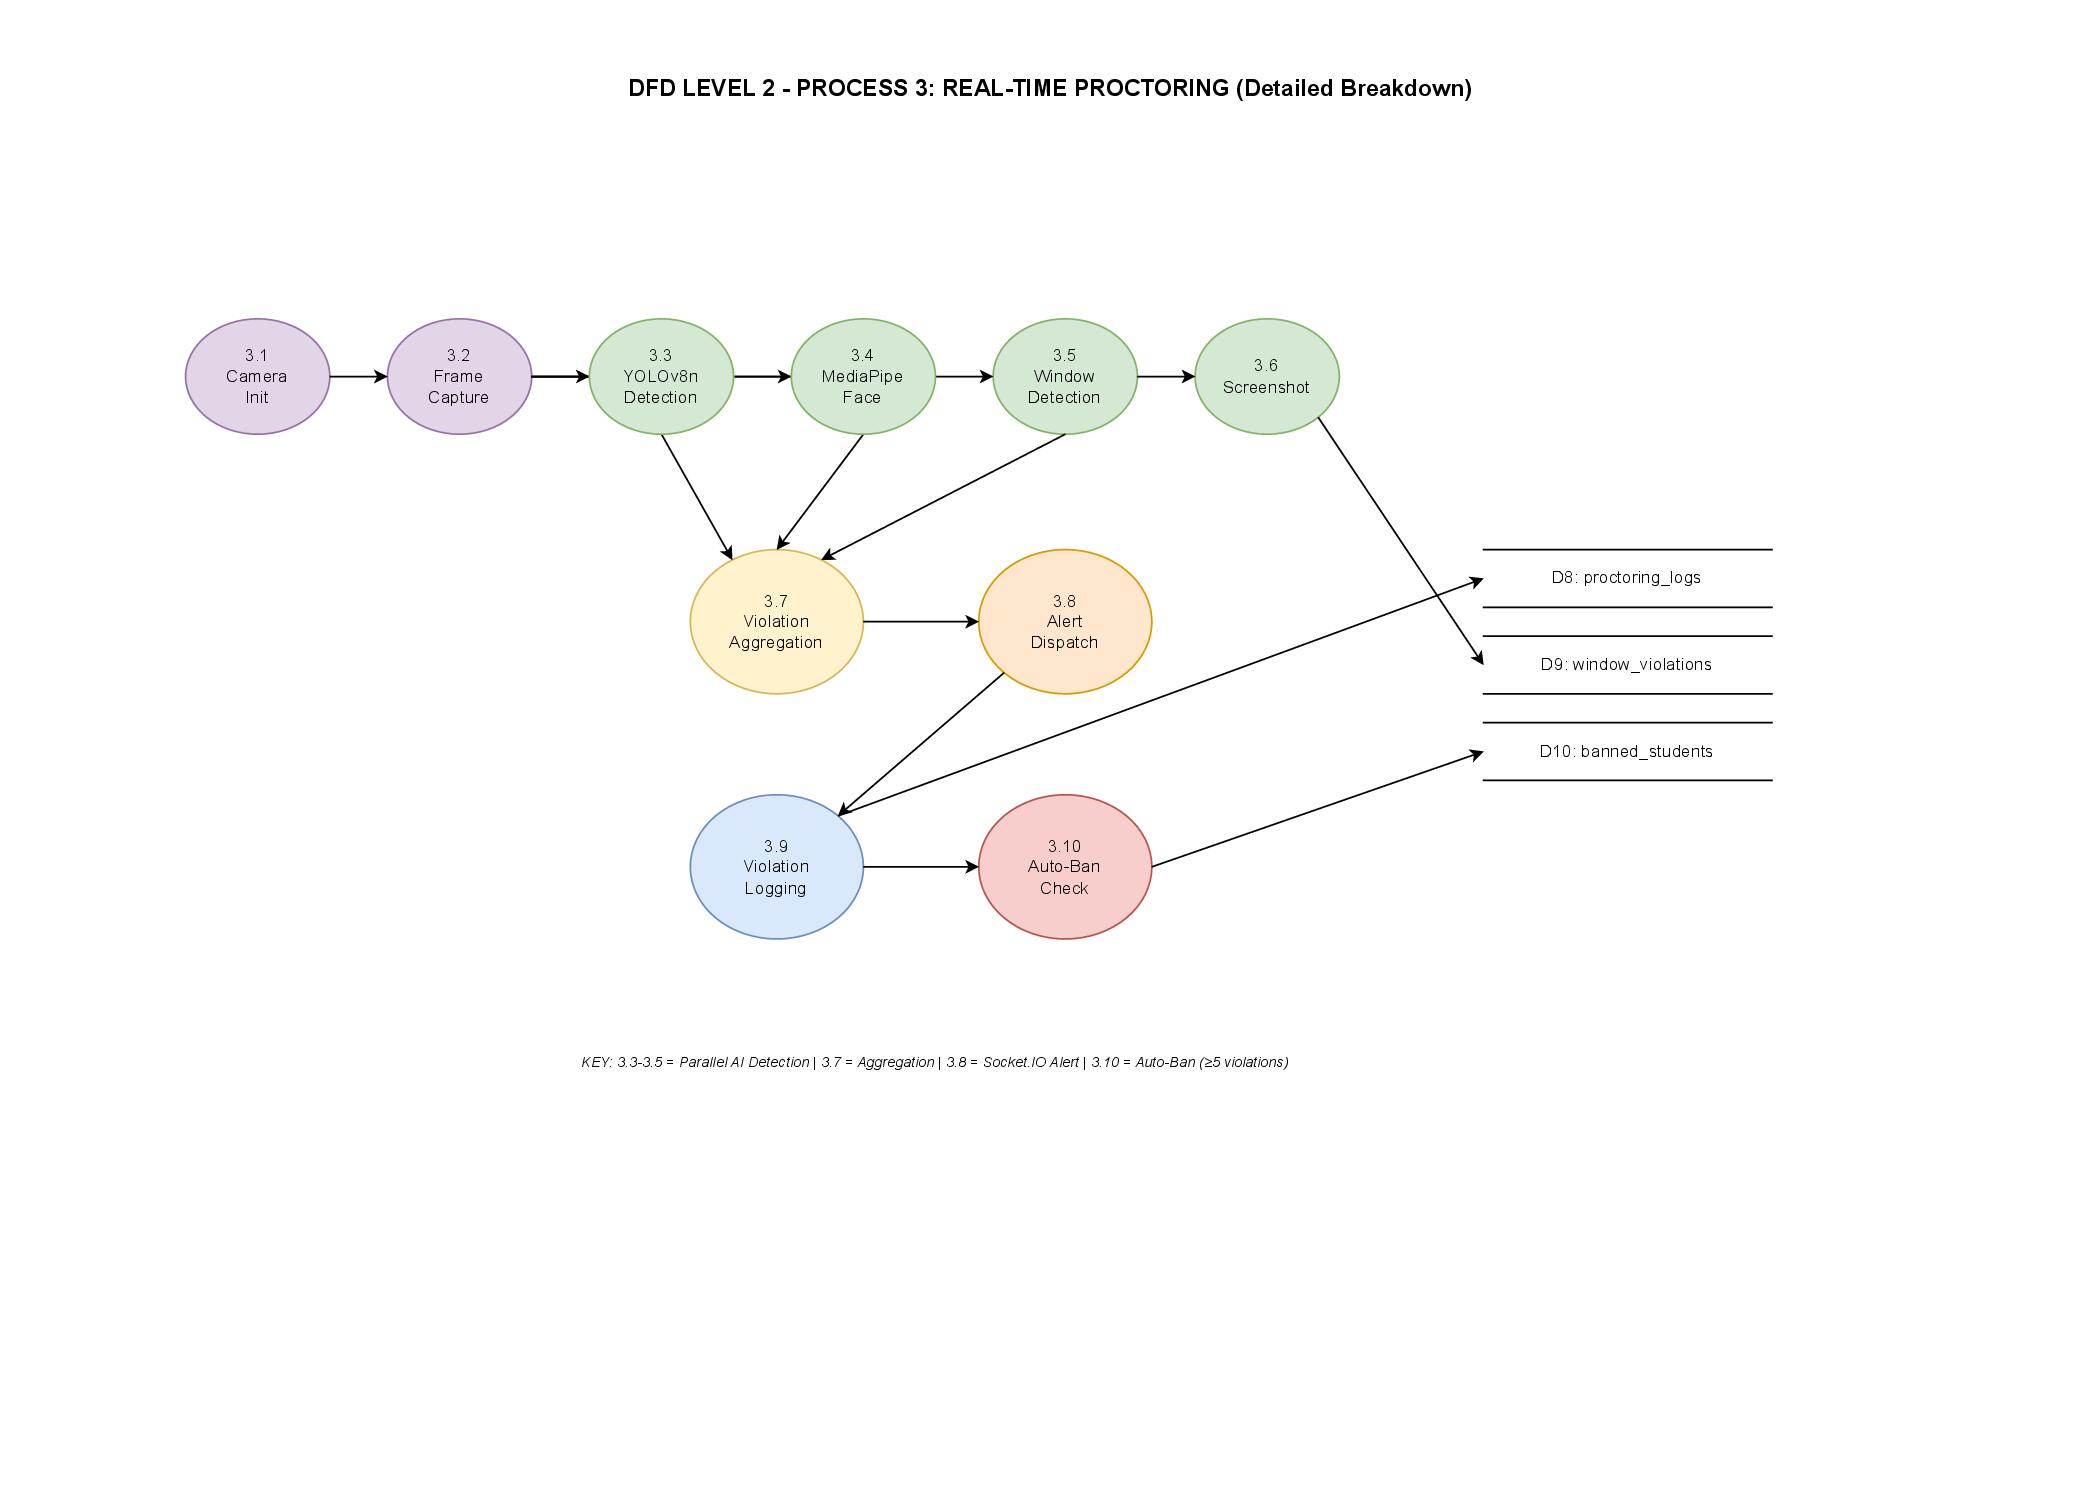
\includegraphics[width=0.85\textwidth]{Chap3/dfd_level2}
    \caption{Data Flow Diagram Level 2 - Real-Time Proctoring Process Decomposition}
    \label{fig:dfd2}

    \vspace{1cm}

    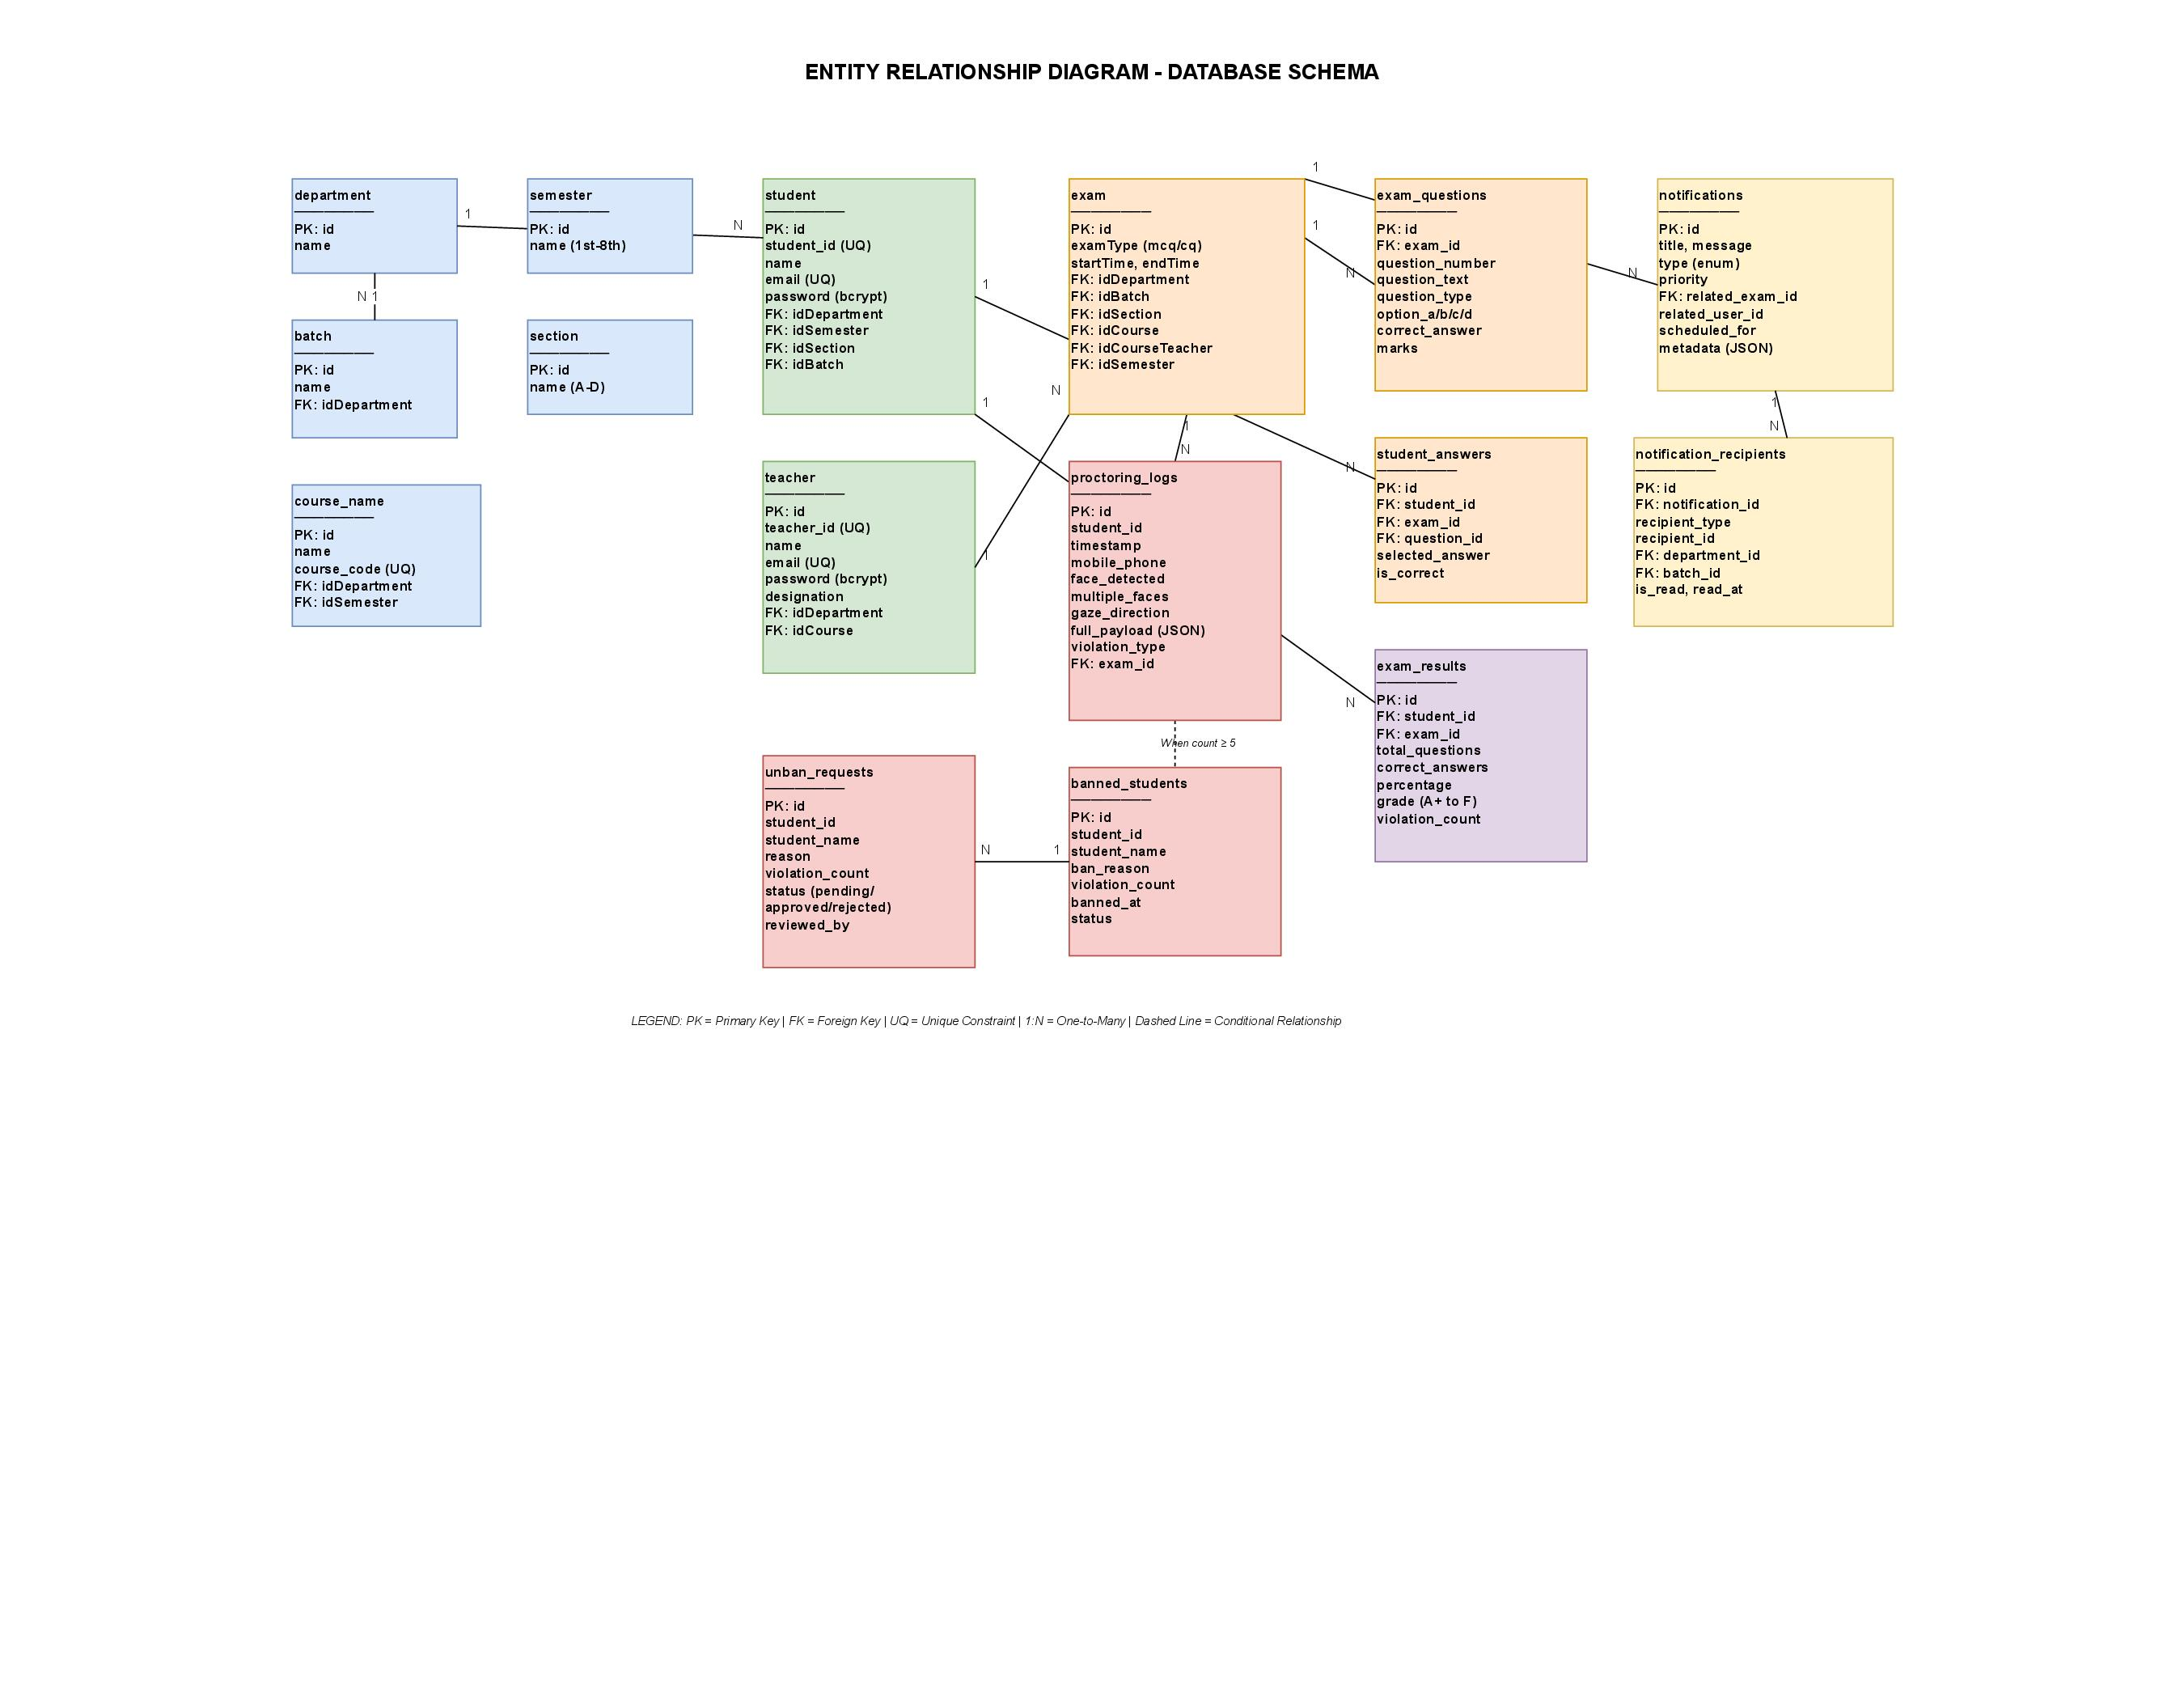
\includegraphics[width=0.85\textwidth]{Chap3/er_diagram}
    \caption{Entity Relationship Diagram - Complete Database Schema (21 Entities)}
    \label{fig:er}
\end{figure}

\section{Database Normalization and Integrity}

The database follows Third Normal Form (3NF): \textbf{1NF} (atomic values, no repeating groups), \textbf{2NF} (all non-key attributes fully depend on PK, partial dependencies eliminated), \textbf{3NF} (no transitive dependencies, academic hierarchy normalized). \textbf{Referential Integrity:} All foreign keys use ON DELETE CASCADE/SET NULL to prevent orphaned records (e.g., deleting exam cascades to exam\_questions, student\_answers, exam\_results, proctoring\_logs). \textbf{Constraints:} CHECK (percentage 0-100), ENUM (question\_type, violation\_type, grade), UNIQUE (email, registration\_no, student\_id+exam\_id), NOT NULL (mandatory fields).

\section{Summary}

This chapter presented comprehensive system design through nine diagrams: flowchart (examination lifecycle), workflow (five-phase parallel activities), use case (four actors with 50+ use cases), activity (concurrent monitoring swimlanes), sequence (temporal message flow), data flow diagrams (three hierarchical levels), and entity relationship diagram (21-table 3NF schema). These artifacts serve as implementation blueprints, ensuring systematic development aligned with functional requirements, security objectives, and scalability goals.
